\section{Reconstructed photon spectrum}

For the photon energy of $\sim$ 130 MeV, the present reconstruction code is not expected
to reconstruct $\gamma \to e^+e^-$ events efficiently.

{\red run reconstruction and demonstrate that ? }

However, the intrinsic resolution of the tracker should contribute less than 0.5 MeV to the
reconstructed full width of the $e^+e^-$ conversion peak.

We therefore use the MC truth - the sum of the two MC particle momenta recorded in front
of the tracker - as a proxy to the reconstructed photon momentum
\begin{figure}[H]
  \begin{tikzpicture}
    \node[anchor=south west,inner sep=0] at (0,0.) {
      % \node[shift={(0 cm,0.cm)},inner sep=0,rotate={90}] at (0,0) {}
      \makebox[\textwidth][c] {
        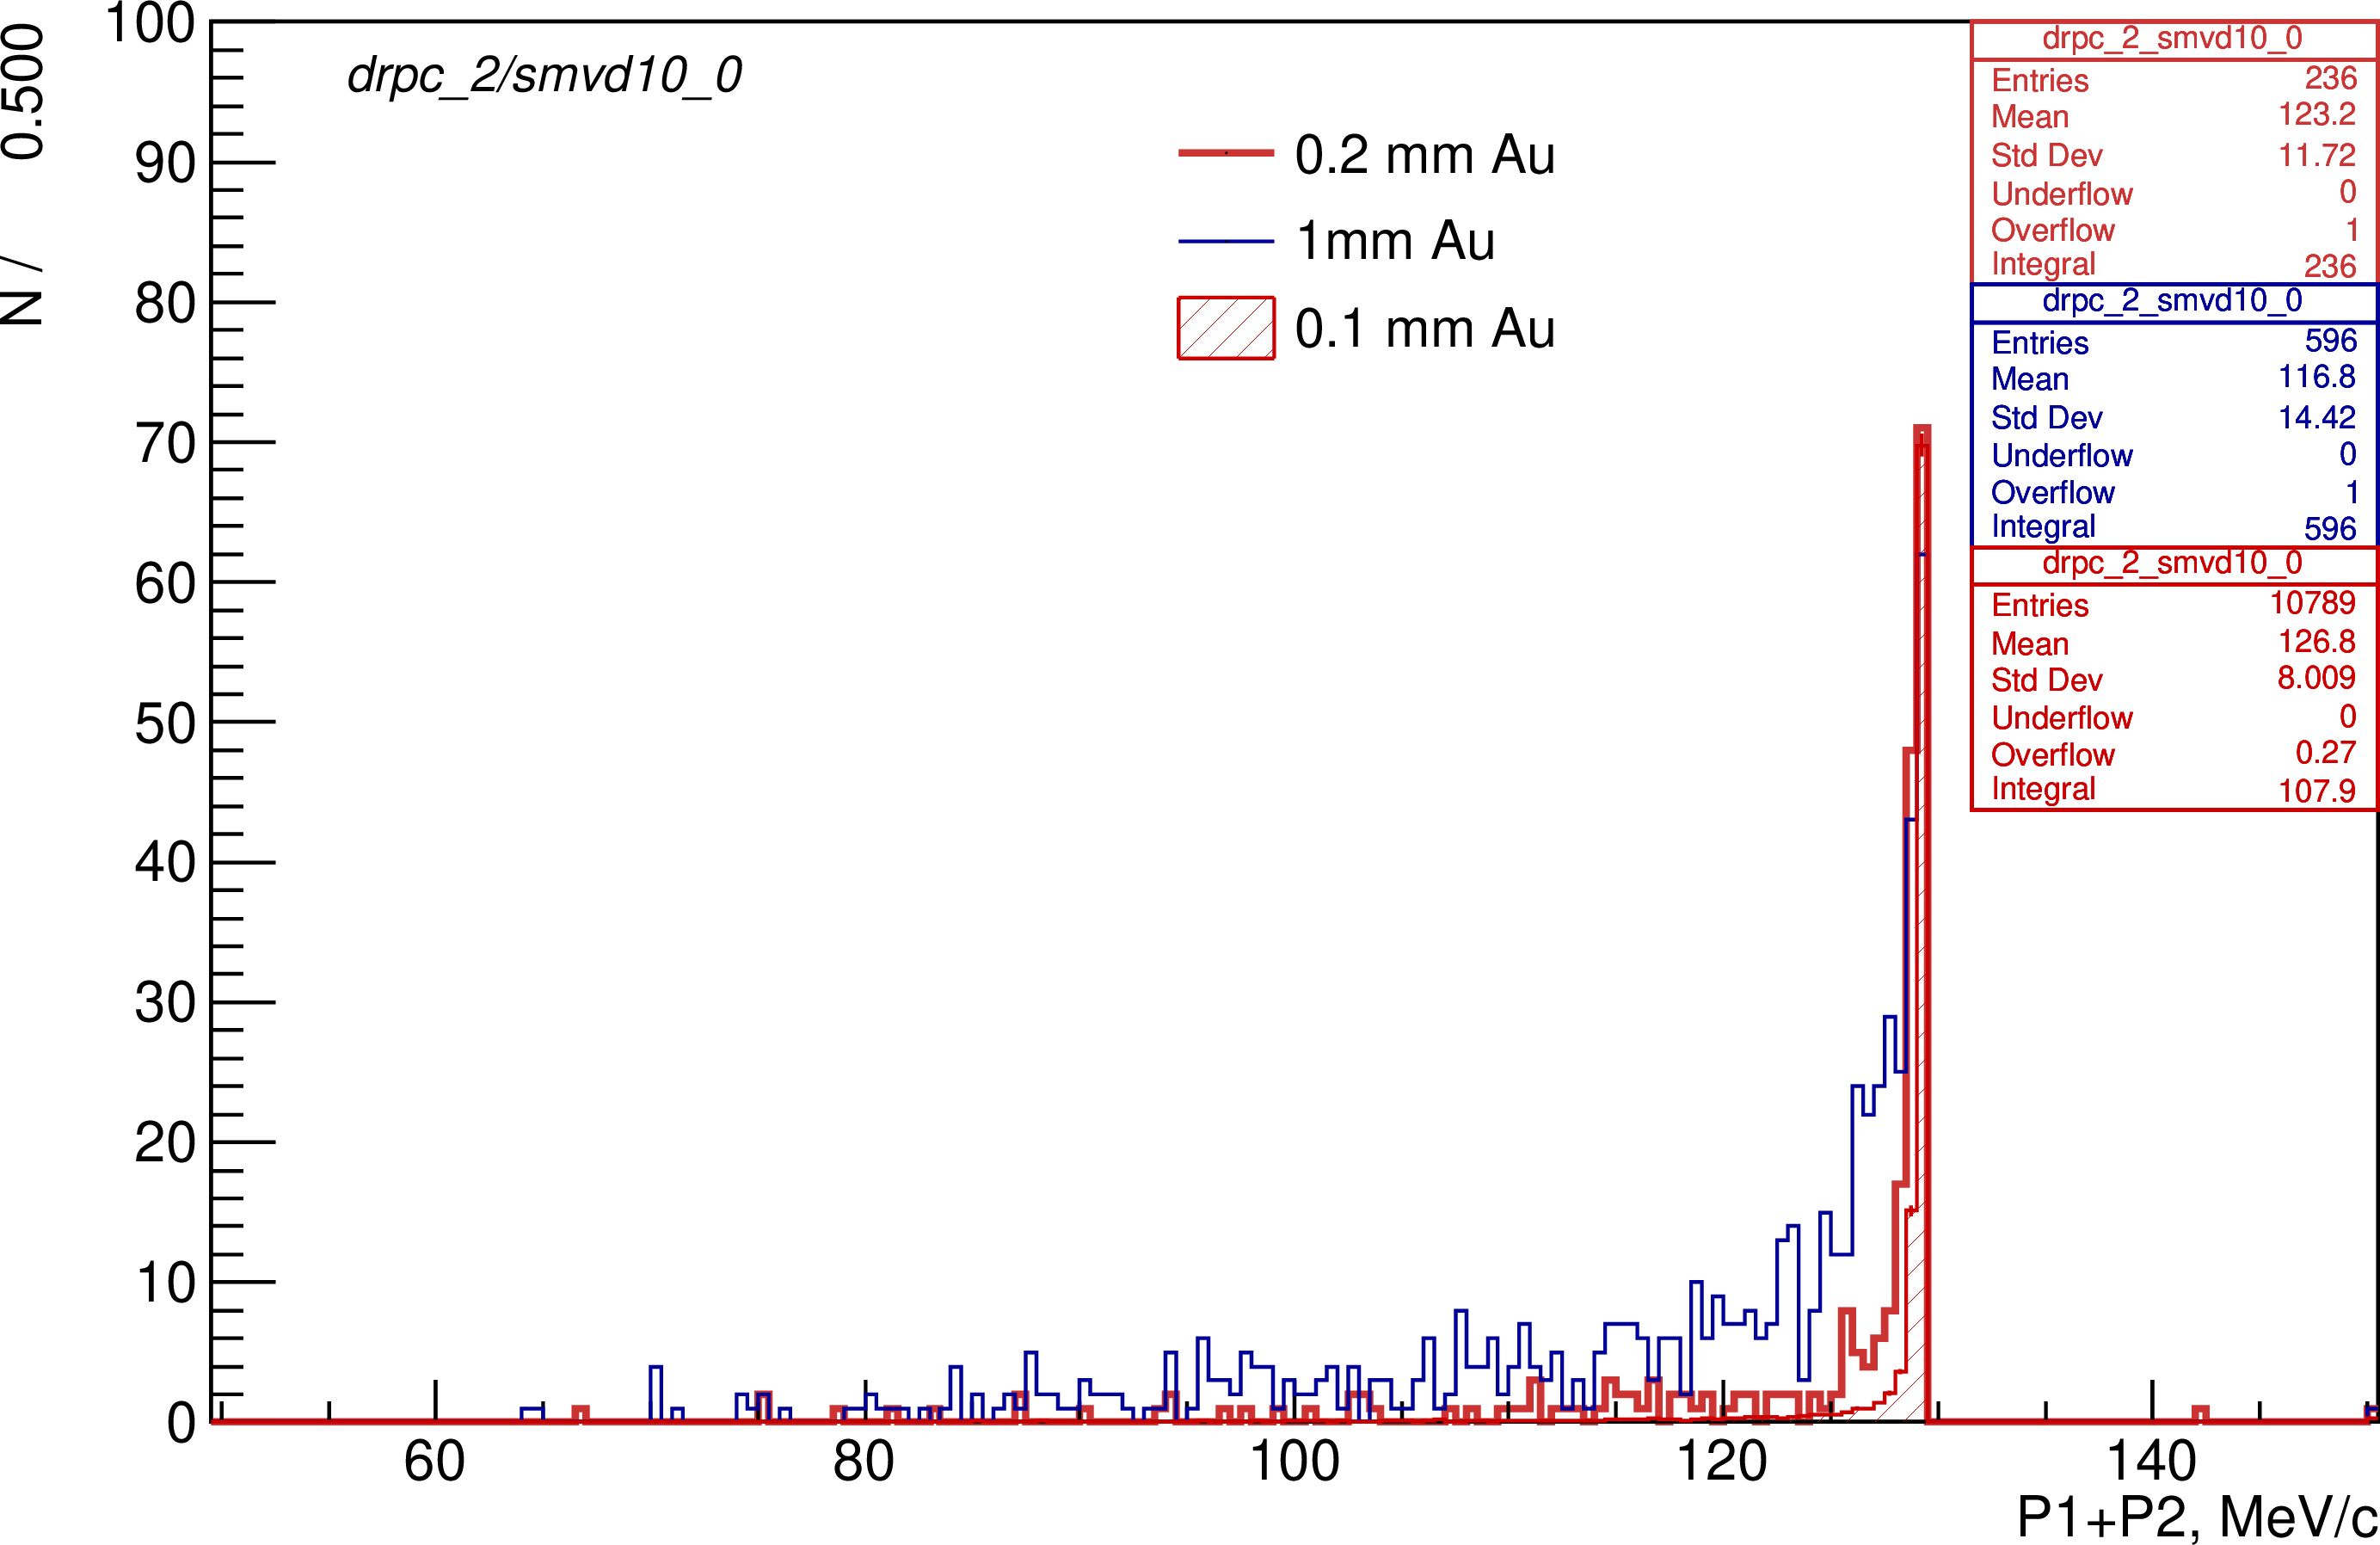
\includegraphics[width=0.9\textwidth]{png/figure_00010}
      }
    };
    % \node [text width=8cm, scale=1.0] at (14.5,0.5) {$\mu_B$, expected background mean};
    % \node [text width=8cm, scale=1.0, rotate={90}] at (1.5,7.5) { $S_{D}$, ``discovery'' signal strength  };
  \end{tikzpicture}
  \caption{
    \label{figure:sum_mom_vd10}
    P1+P2 at VD10
  }
\end{figure}

\begin{figure}[H]
  \begin{tikzpicture}
    \node[anchor=south west,inner sep=0] at (0,0.) {
      % \node[shift={(0 cm,0.cm)},inner sep=0,rotate={90}] at (0,0) {}
      \makebox[\textwidth][c] {
        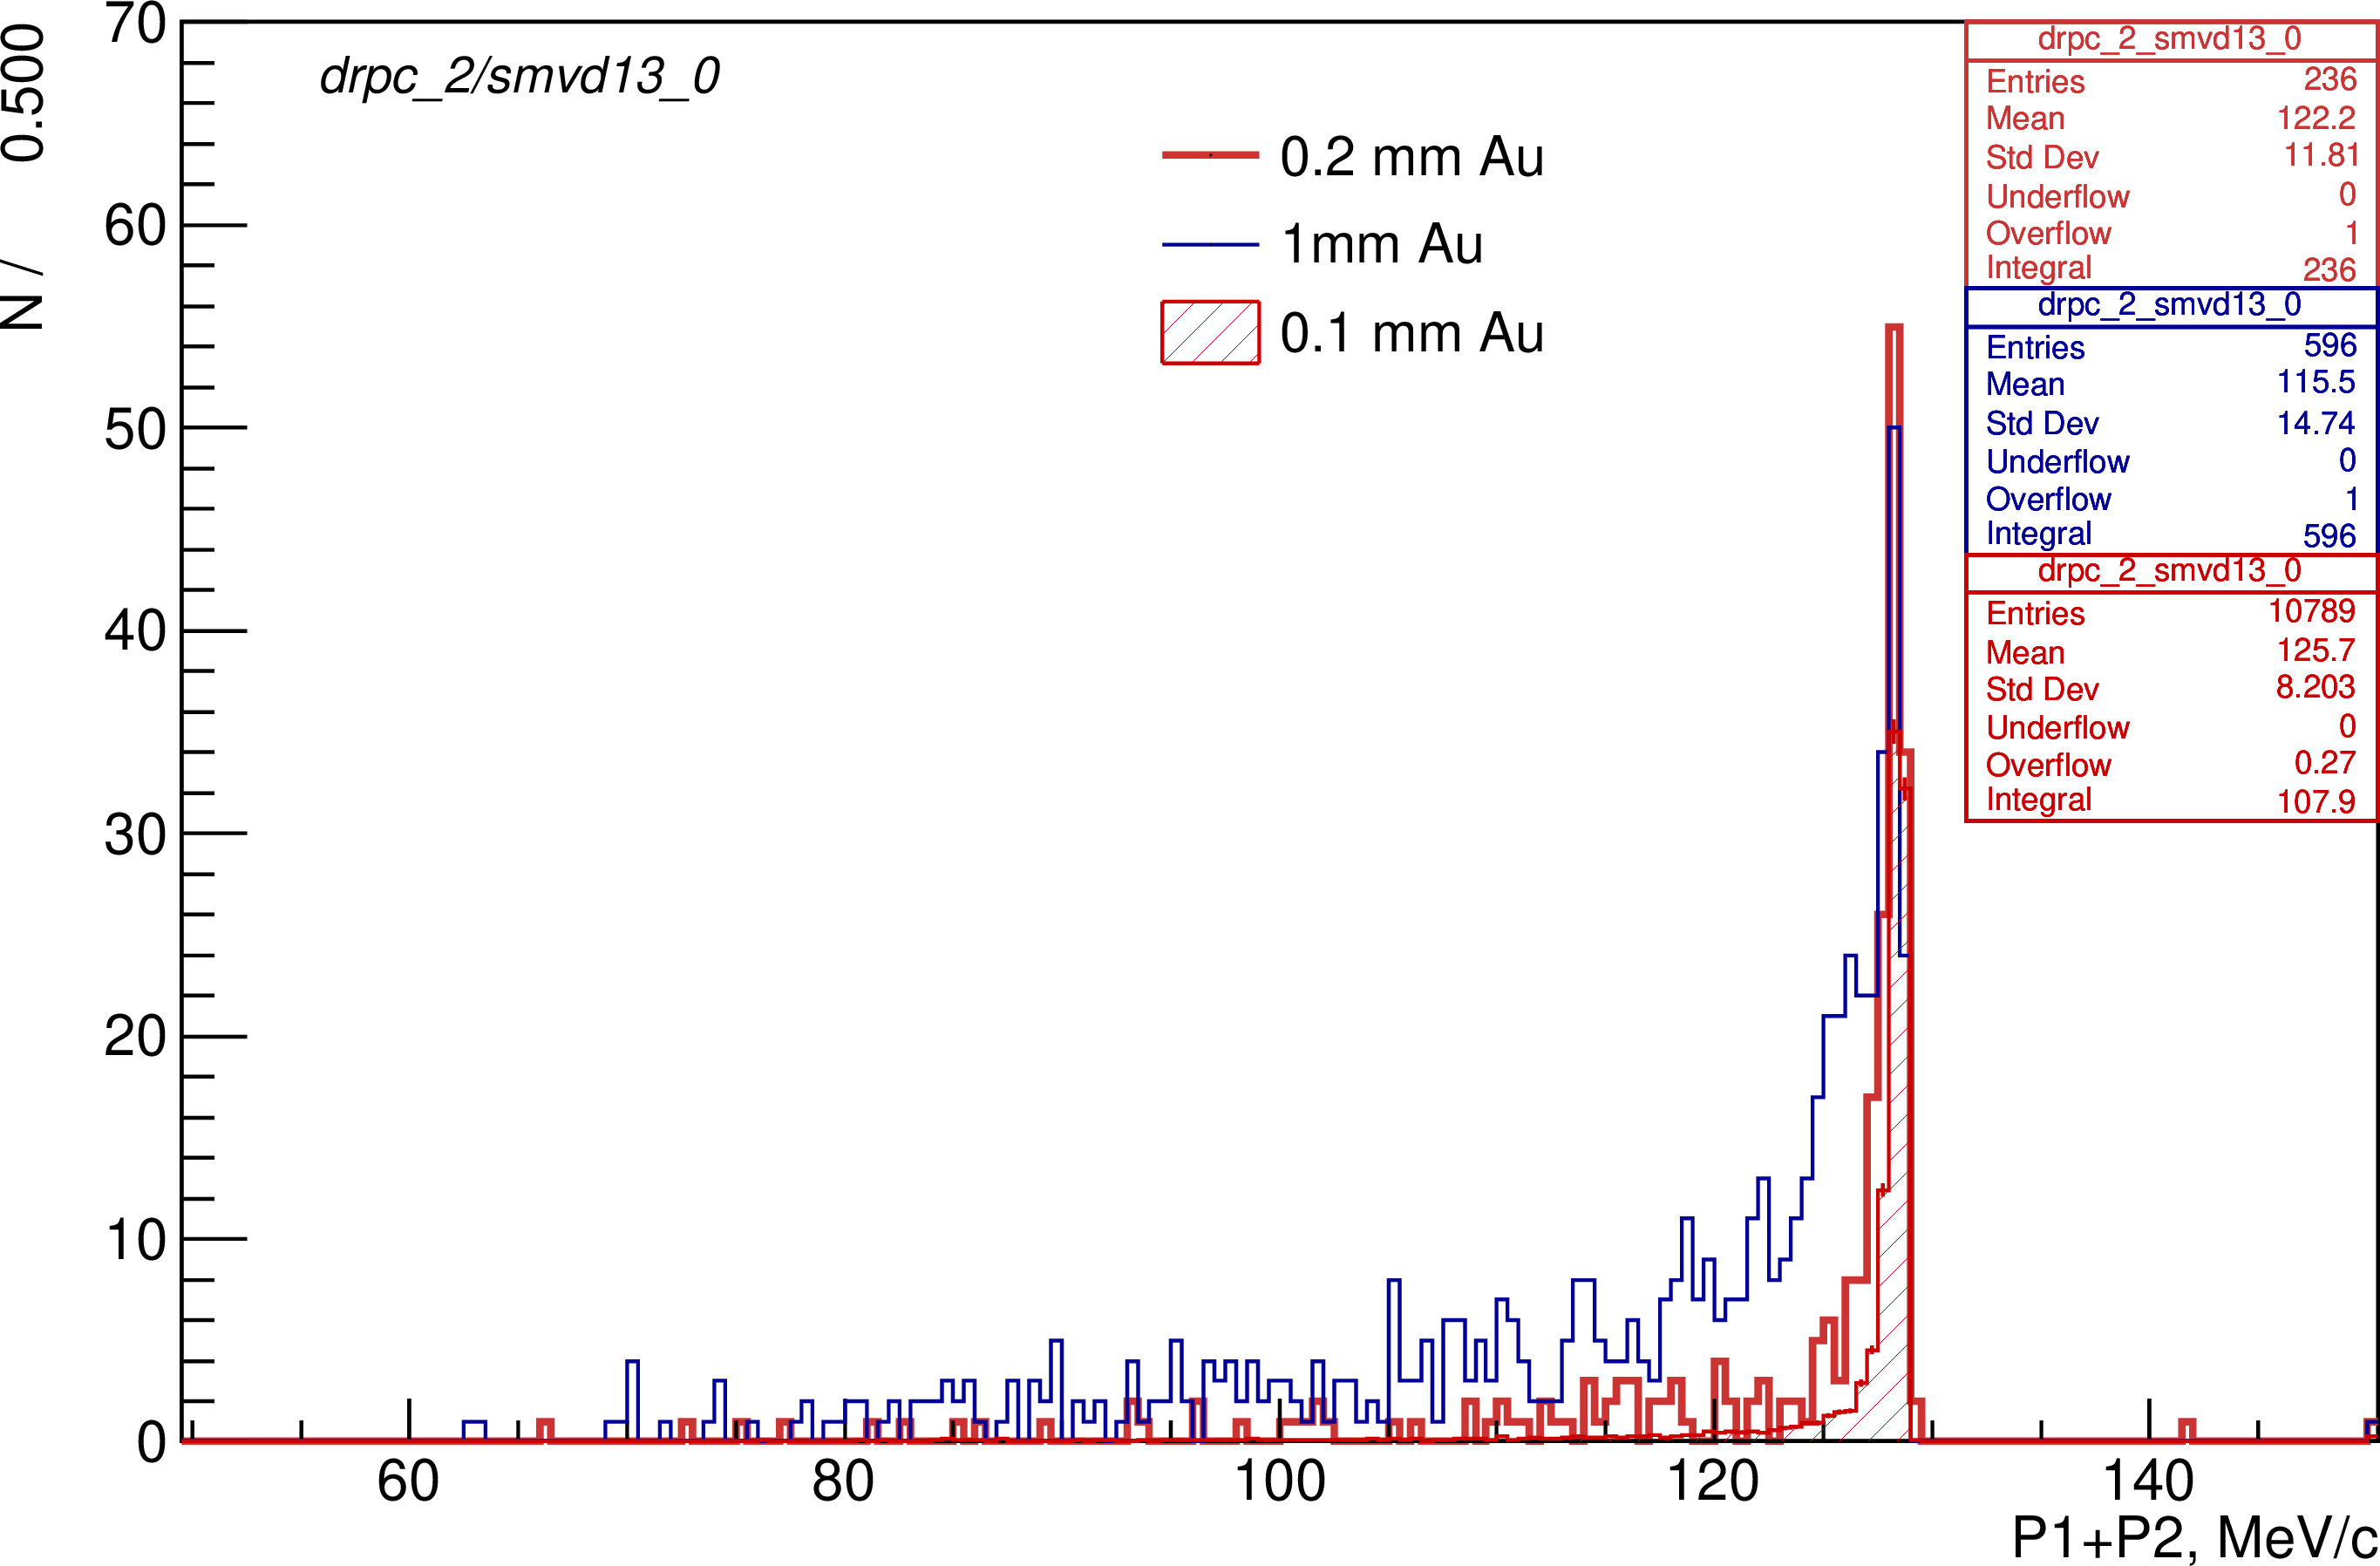
\includegraphics[width=0.9\textwidth]{png/figure_00013}
      }
    };
    % \node [text width=8cm, scale=1.0] at (14.5,0.5) {$\mu_B$, expected background mean};
    % \node [text width=8cm, scale=1.0, rotate={90}] at (1.5,7.5) { $S_{D}$, ``discovery'' signal strength  };
  \end{tikzpicture}
  \caption{
    \label{figure:sum_mom_vd13}
    P1+P2 at VD09, VD10, VD13
  }
\end{figure}

The converter thickness is chosen based on the distributions shown in Figure~\ref{figure:sum_mom_vd13}.
Plotted: $P_{tot} = P_1 + P_2$ at VD13, virtual detector in front of the tracker fro events with
two particles, an electron and a positron with P > 30 MeV/c and producing 20 or more straw hits in the tracker each.
Such particles provide a good proxy to the reconstructable tracks.

The event yield increases with the converter thickness. However of interest for the scale calibration only
are the events close to the kinematic edge.
The highest yield of events with P > 128 Mev/c corresponds to the 100 um gold foil, and that determines
the choice of 100 um thick converter.

\begin{figure}[H]
  \begin{tikzpicture}
    \node[anchor=south west,inner sep=0] at (0,0.) {
      % \node[shift={(0 cm,0.cm)},inner sep=0,rotate={90}] at (0,0) {}
      \makebox[\textwidth][c] {
        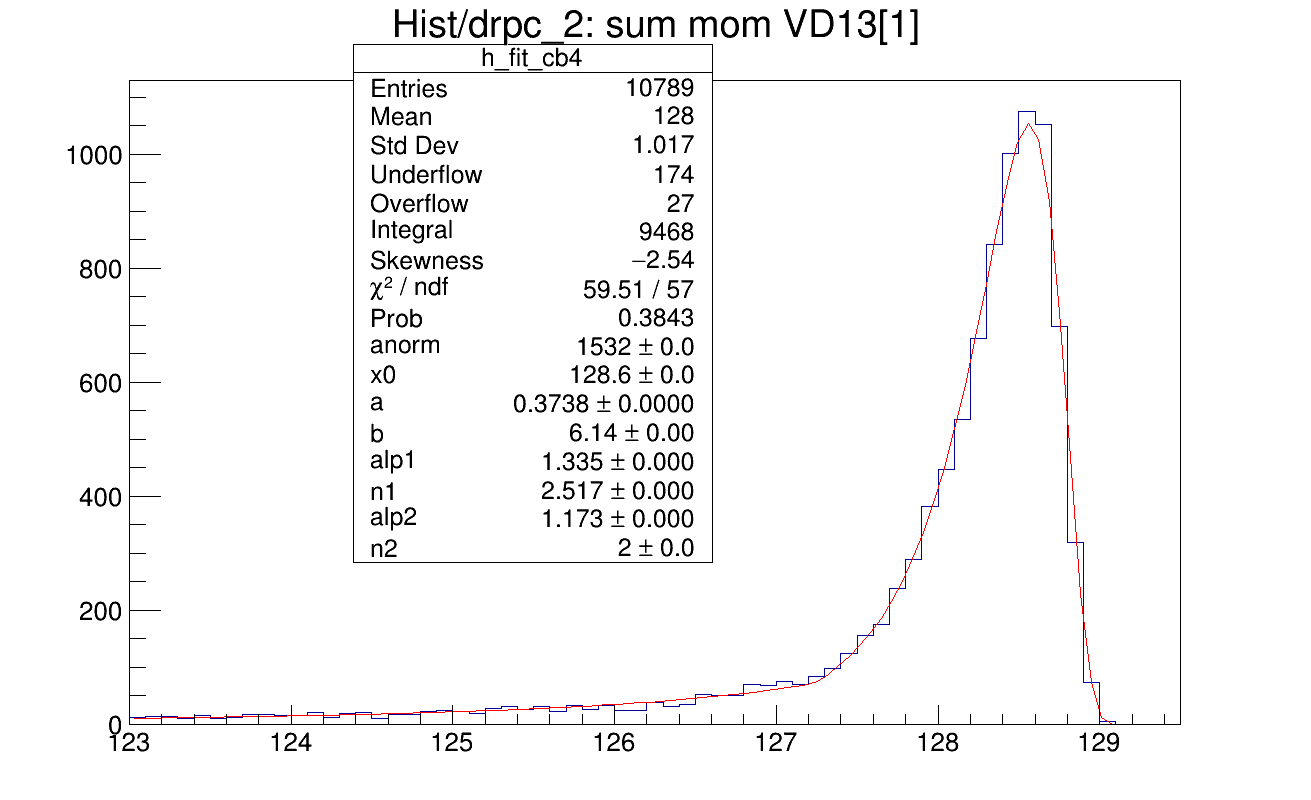
\includegraphics[width=0.9\textwidth]{png/pipenu_bpip4b0_murat_track_ana_trk_0_p_fit}
      }
    };
    % \node [text width=8cm, scale=1.0] at (14.5,0.5) {$\mu_B$, expected background mean};
    % \node [text width=8cm, scale=1.0, rotate={90}] at (1.5,7.5) { $S_{D}$, ``discovery'' signal strength  };
  \end{tikzpicture}
  \caption{
    \label{figure:sum_mom_vd09_10_13}
    P1+P2 at VD09, VD10, VD13
  }
\end{figure}

Figure ~\ref{figure:sum_mom_vd09_10_13} shows the $P_{tot}$ distribution for 100 um converter
with the binning of 100 keV/c. The most probable energy loss is about 800/c keV, 
and the resolution function has the FWHM of about 700 keV/c.
These numbers are not very different from the same numbers for conversion electrons.

Assuming that, similar to the CE case, the width of the distribution is dominated by the energy losses,
the reconstructed $\gamma \to e^+e^-$ peak will have the FWHM $\simeq 1$ MeV/c and the offset
of about 1 MeV from its nominal position.

{\red need fit uncertainties to estimate the uncertainty on the edge position }

%%% Local Variables:
%%% mode: latex
%%% TeX-master: t
%%% End:
